% Drawing 138/06-46 -- folder 138, batch 06, archive page 118 (PDF page 119).
% Transcription: un segment suivi d'une étoile à quatre branches, $\mathbb{Z}_2$ ; un segment suivi d'une étoile avec boucle, $1$ (un $\mathbb{Z}_2$ biffé) ; un segment suivi d'une boucle avec arêtes, $1$ ; un segment suivi d'une boucle à deux arêtes intérieures, $\mathbb{Z}_2$ ; un segment suivi de deux boucles, $\mathbb{Z}_2$ ; deux boucles et une arête terminée par un sommet, $1$ ; au crayon, dans un enclos, une boucle avec segment, $\mathbb{Z}_2$.
% Kind: table of small maps with automorphism groups (degree 6, b). Method 2 (schematic redraw from the facsimile). Status: ok.
% Notes: Degree 6, b): a segment followed by a star with four branches, Z_2; a segment followed by a star with a loop, 1; a segment followed by a loop with edges, 1 (circled); a segment followed by a loop with two inner edges, Z_2; a segment followed by two loops, Z_2; two loops and an edge ending at a vertex, 1 (circled); in pencil, inside an enclosure, a loop with a segment, Z_2. Omitted as struck: the Z_2 scribbled out under the second map (replaced by 1). The ink blot at the left is not a drawing. Each small map carries its automorphism group as written (given as labels, since the transcription names them); vertex positions and loop shapes approximate. Issue 128, 2026-11-09: struck material left out after a fresh check of the facsimile (struck-out material is not drawn). Redrawn 2026-11-09 (issue 128): to check again.
% Coordinates: 1 unit = 1 mm = 1/100 of the crop width (bbox in page fractions: [0.214, 0.297, 0.895, 0.464]).
% Redrawn by Claude (claude-opus-5-5), issue #73, 2026-11-07; not checked by a human; not compiled (no TeX in the session).
% Rights: reproduces part of the work -- behind RENDER_TRANSCRIPTS, never published by itself.
\documentclass[tikz,border=3pt]{standalone}
\usepackage{amsmath,amssymb}
\usetikzlibrary{patterns,arrows.meta}
\tikzset{pencil/.style={black!45}, struck/.style={black!35}, mark/.style={circle,draw,inner sep=1.3pt}, pt/.style={circle,fill,inner sep=0.9pt}, opt/.style={circle,draw,fill=white,inner sep=1.1pt}}
\begin{document}
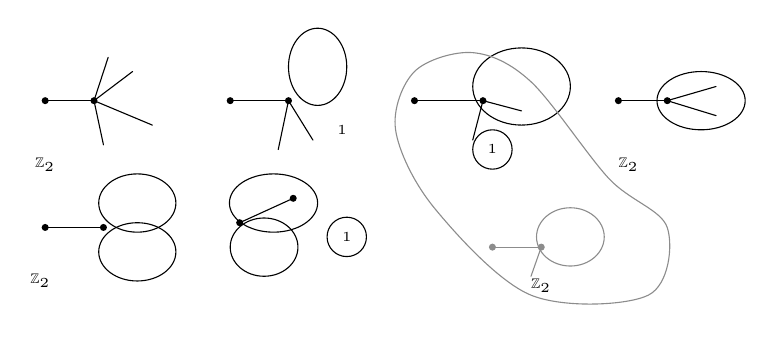
\begin{tikzpicture}[x=1mm,y=1mm,line cap=round,line join=round,font=\scriptsize]
\draw (7.4,-8.6) -- (13.6,-8.6);
\draw (13.6,-8.6) -- (18.5,-4.9);
\draw (13.6,-8.6) -- (21,-11.7);
\draw (13.6,-8.6) -- (14.8,-14.2);
\draw (13.6,-8.6) -- (15.4,-3.1);
\node[pt] at (7.4,-8.6) {};
\node[pt] at (13.6,-8.6) {};
\node[inner sep=1pt] at (7.4,-16.7) {\tiny $\mathbb{Z}_2$};
\draw (30.9,-8.6) -- (38.3,-8.6);
\draw (42,-4.3) ellipse[x radius=3.7, y radius=4.9];
\draw (38.3,-8.6) -- (37,-14.8);
\draw (38.3,-8.6) -- (41.4,-13.6);
\node[pt] at (30.9,-8.6) {};
\node[pt] at (38.3,-8.6) {};
\node[inner sep=1pt] at (45.1,-12.3) {\tiny $1$};
\draw (54.3,-8.6) -- (63,-8.6);
\draw (67.9,-6.8) ellipse[x radius=6.2, y radius=4.9];
\draw (63,-8.6) -- (61.7,-13.6);
\draw (63,-8.6) -- (67.9,-9.9);
\node[pt] at (54.3,-8.6) {};
\node[pt] at (63,-8.6) {};
\draw (64.2,-14.8) circle[radius=2.5];
\node[inner sep=1pt] at (64.2,-14.8) {\tiny $1$};
\draw (80.2,-8.6) -- (86.4,-8.6);
\draw (90.7,-8.6) ellipse[x radius=5.6, y radius=3.7];
\draw (86.4,-8.6) -- (92.6,-6.8);
\draw (86.4,-8.6) -- (92.6,-10.5);
\node[pt] at (80.2,-8.6) {};
\node[pt] at (86.4,-8.6) {};
\node[inner sep=1pt] at (81.5,-16.7) {\tiny $\mathbb{Z}_2$};
\draw (7.4,-24.7) -- (14.8,-24.7);
\draw (19.1,-21.6) ellipse[x radius=4.9, y radius=3.7];
\draw (19.1,-27.8) ellipse[x radius=4.9, y radius=3.7];
\node[pt] at (7.4,-24.7) {};
\node[pt] at (14.8,-24.7) {};
\node[inner sep=1pt] at (6.8,-31.5) {\tiny $\mathbb{Z}_2$};
\draw (36.4,-21.6) ellipse[x radius=5.6, y radius=3.7];
\draw (35.2,-27.2) ellipse[x radius=4.3, y radius=3.7];
\draw (32.1,-24.1) -- (38.9,-21);
\node[pt] at (32.1,-24.1) {};
\node[pt] at (38.9,-21) {};
\draw (45.7,-25.9) circle[radius=2.5];
\node[inner sep=1pt] at (45.7,-25.9) {\tiny $1$};
\draw[pencil] (64.2,-27.2) -- (70.4,-27.2);
\draw[pencil] (74.1,-25.9) ellipse[x radius=4.3, y radius=3.7];
\draw[pencil] (70.4,-27.2) -- (69.1,-30.9);
\node[pt,pencil] at (64.2,-27.2) {};
\node[pt,pencil] at (70.4,-27.2) {};
\node[inner sep=1pt] at (70.4,-32.1) {\tiny $\mathbb{Z}_2$};
\draw[pencil] plot[smooth cycle, tension=0.55] coordinates {(54.3,-4.9) (61.7,-2.5) (69.1,-6.2) (79,-18.5) (86.4,-24.7) (84,-33.3) (69.1,-33.3) (56.8,-22.2) (51.9,-12.3)};
\end{tikzpicture}
\end{document}
